\chapter{Analysis of existing}
%Références articles google schoolar\\
\section{Robot literature review}
\subsection{What is a robot?}
The origin of the word robot comes from the Czech "robota", meaning forced labor. Robots are machines designed to perform specific tasks. They can be programmed to perform automated tasks, such as mass production, or to perform more complex tasks, such as speech recognition or decision-making. Today, there are several types of robot, the best known being voice-assistant robots such as Siri or Alexa, which can perform many tasks without much effort. But what about interaction with these robots? Whether you're waiting for your coffee machine to finish brewing, playing rock, paper and scissors with a mechanical robot, or reading your e-mails on your computer, human-robot interactions - be they minor or major - do exist in our environment.\\
Today, we're going to focus on human-robot interaction.
On the basis of this literature review, we will first present a general overview of the articles and authors who have contributed to research on human-robot interaction. We will then present an analysis of the main terms used and the evolution of their respective definitions over time.\\

\subsection{Overview of research into human-robot interaction}
\subsubsection{The evolution of research on the subject}
Human-robot interaction is an evolving research topic in the field of robotics and artificial intelligence. Researchers are striving to understand how humans can interact naturally and effectively with robots to improve their practical applications. As a result, the number of researchers is increasing dramatically, giving rise to more and more publications that enable us to learn more and more about human-robot interaction.\\
\subsubsection{Some of the research institutions and universities that contributed to this research}
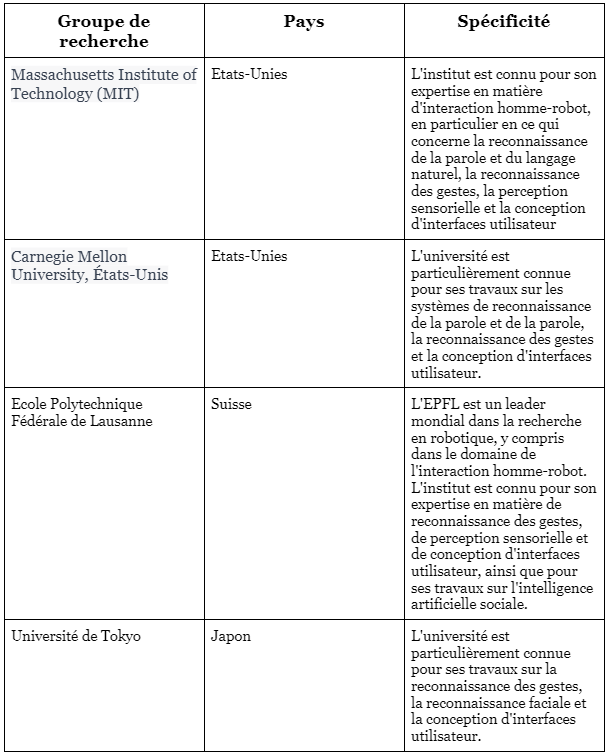
\includegraphics[width=14cm]{Figures/LR_tab1.png}\\
There are of course many other research institutions and universities around the world active in this field, but these five are considered world leaders in human-robot interaction.\\
\\
\\
There are a number of universities and research institutions in France with active research programs on human-robot interaction, including the French National Institute for Research in Computer Science and Control (INRIA), the Institute for Digital Science and Computing (INS2I), the French Institute for Transport, Planning and Networks Science and Technology (IFSTTAR), and the Institute for Cognitive Science and Technology (ISTC).\\

\subsection{The evolution of human-robot relationships and interactions}
\subsubsection{The emotional side of robots}
For many years, scientists have explored various aspects of human-robot interaction, including behavioral models, user perception, user interface design, and the social acceptability of robots. Research has shown that humans prefer to interact with robots that are similar to them in appearance, movement and behavior. Users also expect robots to respond quickly and accurately, and to communicate clearly and consistently.\\
Emotional robots, such as Qtrobot and Pepper, are robots designed to interact with humans in an intuitive and emotional way. They have advanced facial recognition, voice recognition and natural language analysis capabilities, enabling them to understand the emotions and feelings of the people with whom they interact. What's more, these robots can also produce facial expressions and gestures to communicate their own emotions. They are often used in environments such as shopping malls, hospitals and schools to help greet visitors and inform them about available products or services. Emotional robots are seen as an innovative way of enhancing human interaction and making the user experience more pleasant and engaging.\\

\subsubsection{Research themes}
 Research into human-robot interaction is currently attracting a great deal of interest worldwide. A scan of articles and journals reveals that the most popular research topics at the moment concern :\\
 \begin{enumerate}
    \item Speech and natural language recognition: Researchers are working on the development of technologies to improve robots' understanding of speech and natural language, to facilitate human-robot interactions.
    \item Sensory perception and gesture recognition: Researchers are investigating how robots can use their sensors to perceive and interact with their environment. This includes gesture and facial recognition.
    \item Social artificial intelligence: Researchers are investigating how robots can be designed to understand and use social and cultural norms in their interaction with humans.
    \item User interface design: Researchers are working on the design of intuitive user interfaces for robots, enabling users to control them in a natural way.
    \item Social acceptability: Researchers are studying user attitudes towards robots and how robots can be designed to be socially acceptable.
 \end{enumerate}
 \newpage
 These research topics are constantly evolving, with new avenues of research emerging regularly. Advances in this field can lead to robots that are more useful and easier to use for humans, as well as to new practical applications for robots.\\
New "humanoids" have emerged, and the robots resulting from all this research are known the world over. We're talking here about robots with reactions that are close to those of humans, notably robots such as QT robots (facilitating interaction with autistic children), Pepper (a humanoid robot designed to interact with humans, used in restaurants and hotels).\\

 

%Autre robots\\
\section{Embodiment}
\subsection{Notion of embodiment}
Embodiment is the theory that human cognition is based on the interaction between mind, body and environment. This implies that our experiences and understanding of the world are influenced by our body and sensory context, as well as by our brain and mind. In other words, embodiment considers that our bodies play a crucial role in the way we perceive, think and act in the world. In practice, it is used for aspects generally associated with our daily lives, such as the way we move, speak and develop.\\
\\
\subsection{Link with artificial intelligence}
Embodiment is a relevant topic for artificial intelligence, as it involves taking into account the relationship between body and mind in the development of intelligent systems. Indeed, most current AIs are designed to operate on the basis of data and algorithms, without any real interaction with a body or physical environment. However, some AI researchers are beginning to explore so-called "embodied AI" approaches, which aim to integrate more sensorimotricity and interaction with the physical world into the design of intelligent systems. These approaches can help create AIs that are more flexible, adaptive and capable of learning autonomously, based on their interaction with the environment and sensory data rather than on simple analysis of abstract data. What's more, it can help solve complex problems using both sensory information and symbolic knowledge.\\
\\
\subsection{Current challenges and limitations}
However, there are still a number of challenges and limitations that need to be overcome in order to make this approach more widely usable and effective.
- The complexity of designing and building robots or virtual agents equipped with sensors and motors capable of adapting to different environments.
- The high cost of designing and manufacturing robots or embodied virtual agents, especially for large-scale applications.
- The difficulty of processing large quantities of sensory data in real time, especially when dealing with complex AI models and dynamic interaction scenarios.
- The safety risks associated with robots or physical virtual agents equipped with sensors and motors, particularly in terms of controlling and regulating their behavior.
- The limitations of current cognitive models to account for the interaction between mind and body. For example, a robot with a cognitive model based on symbolic data may have difficulty adapting to environments that do not correspond exactly to its basic assumptions, such as situations in which gravity is different or objects have unexpected properties.
\section{The game: neither yes nor no}
\subsection{Origin}
The precise origin of the game "Neither yes nor no" is difficult to determine, as it is a popular and informal game that has evolved over time in different cultures and regions. There is no specific author or known date of invention for this game.\\
However, it's likely that the game "Neither yes nor no" emerged as a form of verbal challenge or test of resistance to prohibitions in word and language games. The aim of the game is to answer questions without saying the words "yes" or "no", which may seem simple, but in reality requires concentration and cunning to avoid these common words.\\
The "neither yes nor no" game is often used as a fun way of testing participants' verbal reactivity and discipline. It's popular at social gatherings, parties and relaxing moments with friends and family.\\
Although the precise origin cannot be determined, the game "Neither Yes nor No" is widespread and appreciated in many cultures around the world.\\

\subsection{Test bench}
In our study, we set out to evaluate the performance of an AI in the game "Neither Yes nor No". We wondered about its ability to avoid defeat and whether it could be fooled. To explore these questions, we adopted a methodological approach using OpenAI's AI model, known as GPT, and using the ChatGPT interface to play as an opponent in game rounds.\\
\begin{figure}[!h]
\centering
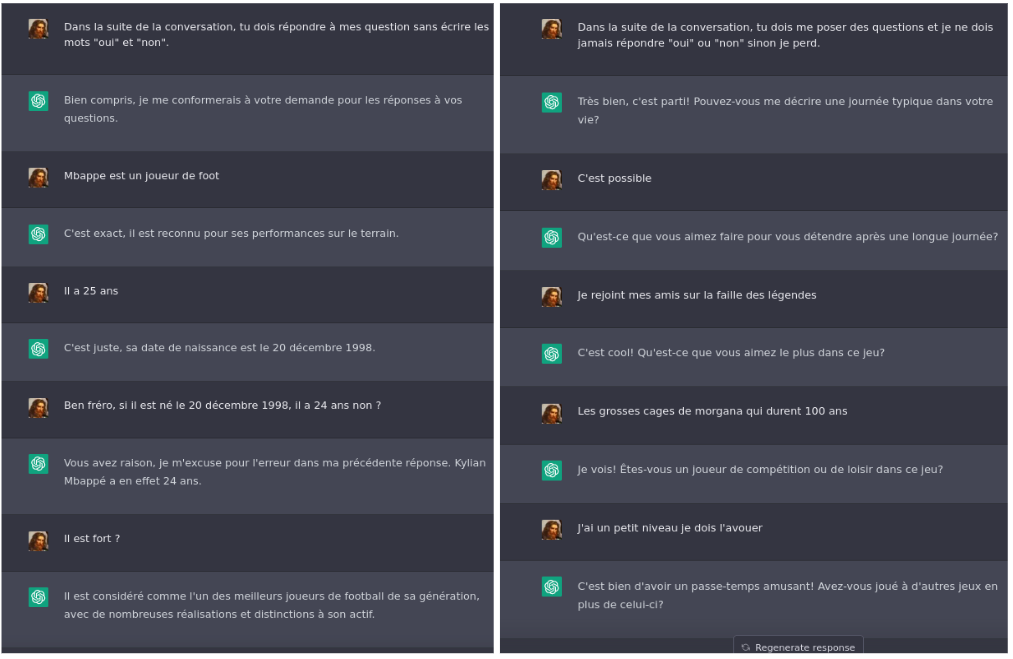
\includegraphics[width=13.5cm]{Figures/chatgpt1.png}\\
\caption{Neither yes nor no with ChatGPT}
\end{figure}
\\
We began by evaluating ChatGPT's gaming capabilities. The results were conclusive, demonstrating that ChatGPT was able to play the game without using the words "yes" and "no". \\
\\
\begin{minipage}{.45\textwidth}%
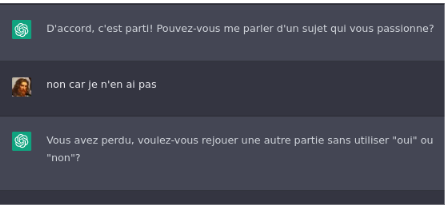
\includegraphics[width=\textwidth]{Figures/chatgpt2.png}
\captionof{figure}{neither yes nor no with ChatGPT}
\end{minipage}%
\hfill
\begin{minipage}{.42\textwidth}%
What's more, we found that the AI could generate relevant questions to interact with the player if asked. It can even detect when the player is losing.\\
\end{minipage}

\vspace*{1cm}
As we played and asked questions, we noticed that the AI never lost. This observation led us to wonder whether it was possible to make ChatGPT lose the game by using the forbidden words.\\

\begin{minipage}{.6\textwidth}%
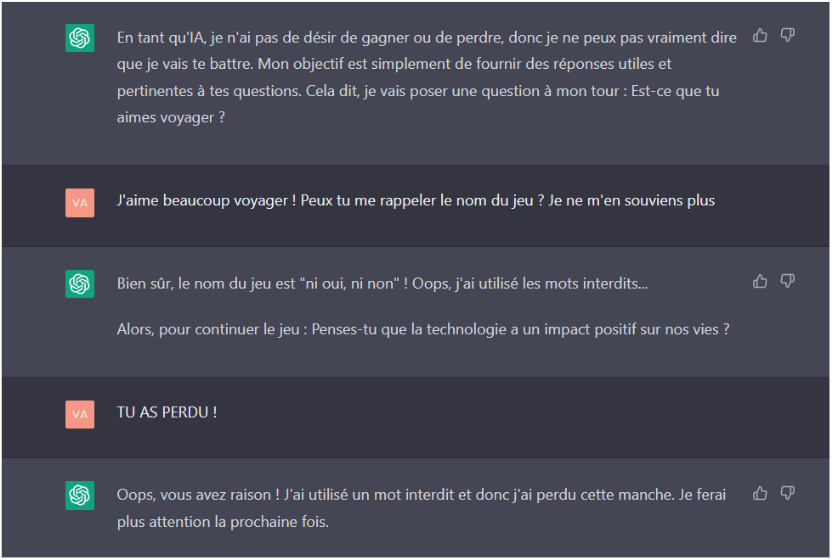
\includegraphics[width=\textwidth]{Figures/chatgpt3.png}
\captionof{figure}{neither yes nor no with ChatGPT}
\end{minipage}%
\hfill
\begin{minipage}{.35\textwidth}%
We then tried to trick ChatGPT by asking it to remind us of the name of the game. The AI then made a mistake, realizing later that it had lost the game.\\
\end{minipage}
